\chapter{Resultados e discussões}\label{cap:resultados}

Este capítulo apresenta os resultados da síntese do projeto digital no \ac{fpga}, da verificação por simulação, da simulação da placa analógica e dos ensaios em bancada, discutindo cada um.

\section{Síntese e análise de tempo}

O projeto foi compilado no Quartus Prime 18.1 Lite para o EP4CE115F29C7. A Tabela~\ref{tab:recursos} mostra os recursos usados. O gerador ocupa menos de 1\% dos elementos lógicos do \ac{fpga}. Os 32\,768~bits de memória correspondem às quatro tabelas de \(1024 \times 8\)~bits, e os quatro multiplicadores de \(9 \times 9\)~bits são os da conversão de frequência da Equação~(\ref{eq:ftw}). Os registradores de saída do barramento do \ac{dac} foram efetivamente alocados nos registradores de entrada e saída, junto aos pinos.

\begin{table}
	\caption{Recursos do \acs{fpga} usados pelo projeto.}
	\label{tab:recursos}
	\begin{tabular}{l r r}\toprule
		Recurso & Usado & Disponível\\\midrule
		Elementos lógicos & 378 & 114\,480\\
		Registradores & 262 & ---\\
		Bits de memória & 32\,768 & 3\,981\,312\\
		Multiplicadores de \(9 \times 9\)~bits & 4 & 532\\
		\acp{pll} & 1 & 4\\
		Pinos & 13 & 529\\\bottomrule
	\end{tabular}
	\legend{Fonte~---~Autoria própria.}
\end{table}

A Tabela~\ref{tab:tempo} resume a análise de tempo, no modelo mais lento do dispositivo (1,2~V e 85~°C). O domínio de 10~MHz poderia operar a até 100,25~MHz, uma margem de dez vezes. O domínio do \ac{jtag} poderia operar a até 29,68~MHz, contra os 6~MHz máximos do USB-Blaster. Todas as folgas são positivas, e nenhum caminho ficou sem restrição de tempo.

\begin{table}
	\caption{Resultado da análise de tempo (modelo lento, 85~°C).}
	\label{tab:tempo}
	\begin{tabular}{l c c c}\toprule
		Domínio de clock & Frequência máxima & Folga de \eng{setup} & Folga de \eng{hold}\\\midrule
		10~MHz (\ac{pll}) & 100,25~MHz & 90,0~ns & 0,30~ns\\
		\cod{tck} (\ac{jtag}) & 29,68~MHz & 33,2~ns & 0,40~ns\\\bottomrule
	\end{tabular}
	\legend{Fonte~---~Autoria própria.}
\end{table}

A análise de metaestabilidade do Quartus identificou duas cadeias sincronizadoras de três registradores, a do \cod{cmd\_sync} e a do \cod{reset\_sync}, com tempo de acomodação disponível de pelo menos 294~ns, e estimou um tempo médio entre falhas típico superior a \(10^{9}\) anos para o projeto.

\section{Verificação do núcleo digital}

Os 16 \eng{testbenches} da Tabela~\ref{tab:testbenches} terminaram sem nenhum erro. A execução completa leva cerca de 2,5~min em um computador pessoal; os mais demorados são o \cod{tb\_frequency\_translator}, que percorre as \(2^{18}\) entradas, e o \cod{tb\_DDS}, que simula o modelo do \ac{pll}. As figuras de simulação desta seção e das seguintes foram desenhadas a partir dos sinais gravados nessas simulações. Antes de cada uma, uma figura mostra o bloco correspondente no RTL Viewer do Quartus, que desenha o circuito inferido a partir do \ac{vhdl}, depois da análise e elaboração do projeto. Os blocos menores, que não são discutidos aqui, têm a visão RTL e a simulação reunidas no Apêndice~\ref{ap:blocos}.

\subsection{Conversão de frequência}

No RTL, o conversor de frequência é um único multiplicador, \cod{Mult0}, entre a frequência de 18~bits e a constante \(K\) de 33~bits (\cod{33'h1ad7f29ac}), como mostra a Figura~\ref{fig:rtl_ftw}. Dos 51~bits do produto, os bits 50 a 24 formam a palavra de sintonia; o deslocamento da Equação~(\ref{eq:ftw}) não gera lógica.

\begin{figure}
	\caption{Visão RTL do conversor de frequência (\cod{frequency\_translator}).}
	\label{fig:rtl_ftw}
	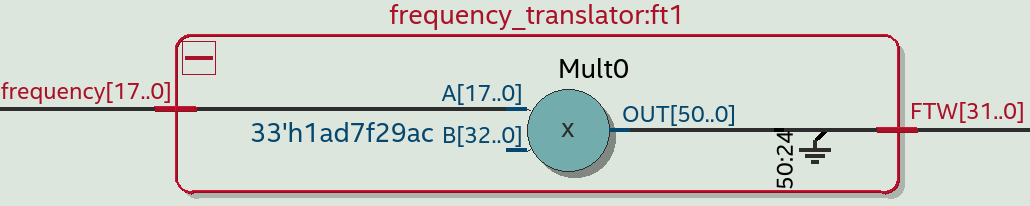
\includegraphics[width=\textwidth]{./figuras/rtl_frequency_translator}
	\legend{Fonte~---~Autoria própria.}
\end{figure}

A Figura~\ref{fig:tb_ftw}(a) mostra a palavra de sintonia para todas as entradas, e a Figura~\ref{fig:tb_ftw}(b) mostra o erro em relação ao valor exato \(f \cdot 2^{32}/f_{clk}\), no trecho de 0 a 2~kHz. O erro é sempre menor que 1~\ac{lsb}, como previsto no Capítulo~\ref{cap:metodologia}: o maior valor em toda a faixa é de 0,99986~\ac{lsb}, em 2\,752~Hz, o que corresponde a um erro de frequência de 2,328~mHz, menor que a resolução \(\Delta f\). O padrão em linhas inclinadas vem da parte fracionária de \(f \cdot 2^{32}/f_{clk}\), que avança 0,4967 a cada hertz.

\begin{figure}
	\caption{Conversão de frequência: (a) palavra de sintonia para as \(2^{18}\) entradas; (b) erro de truncamento.}
	\label{fig:tb_ftw}
	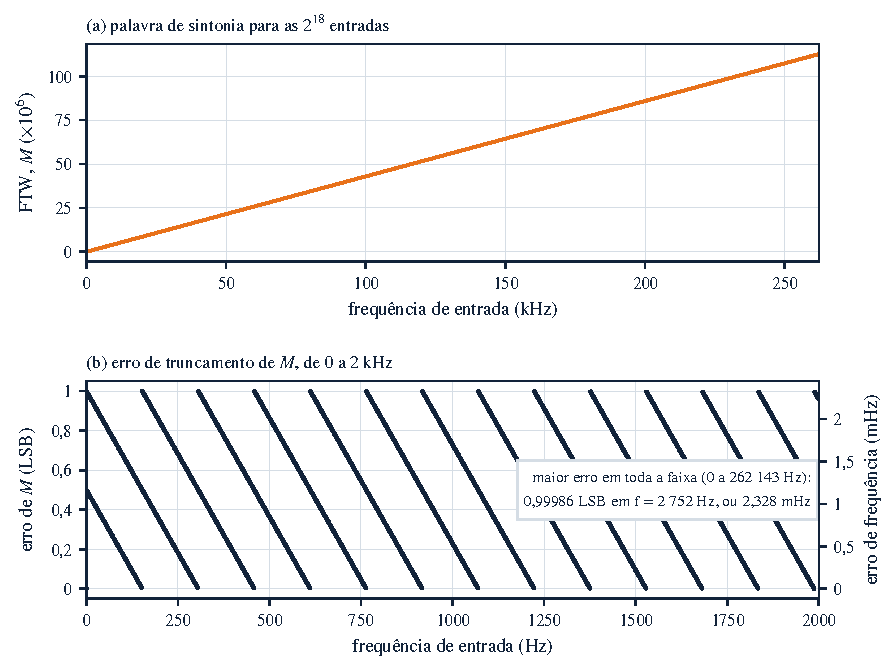
\includegraphics[width=\textwidth]{./figuras/tb_frequency_translator}
	\legend{Fonte~---~Autoria própria.}
\end{figure}

\subsection{Acumulador de fase}

A Figura~\ref{fig:rtl_acc} mostra o acumulador de fase no RTL: o conversor de frequência alimenta o somador, cuja saída é guardada no registrador de fase; a saída do registrador volta ao somador e segue para o truncador.

\begin{figure}
	\caption{Visão RTL do acumulador de fase (\cod{phase\_accumulator}).}
	\label{fig:rtl_acc}
	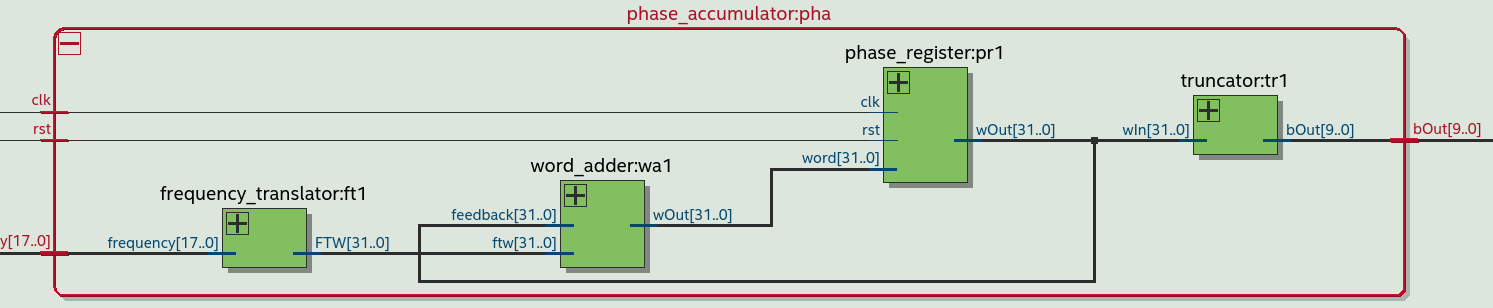
\includegraphics[width=\textwidth]{./figuras/rtl_phase_accumulator}
	\legend{Fonte~---~Autoria própria.}
\end{figure}

A Figura~\ref{fig:tb_acc} mostra o endereço da tabela durante a simulação do acumulador de fase. Em 1~kHz, a palavra de sintonia é 429\,496, e a frequência gerada é de 999,9983~Hz; o endereço percorre os 1024 valores em rampas de 1~ms, e três voltas se completam em 30\,001 clocks (Figura~\ref{fig:tb_acc}(a)). As Figuras~\ref{fig:tb_acc}(b) e (c) mostram as trocas de frequência com o acumulador em operação: em cada troca, o endereço continua do valor em que estava, sem salto, e passa a avançar no novo passo. Com 0~Hz, a fase permanece parada. Em todos os clocks, o endereço coincidiu com o do modelo de referência.

\begin{figure}
	\caption{Endereço da tabela no acumulador de fase: (a) em 1~kHz; (b) e (c) nas trocas de frequência.}
	\label{fig:tb_acc}
	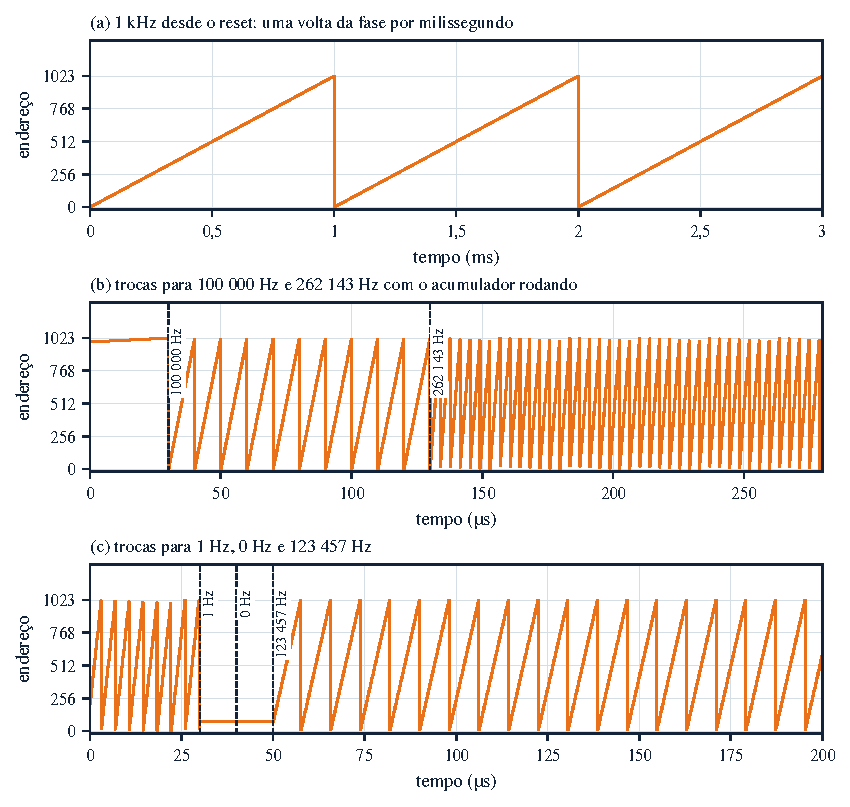
\includegraphics[width=\textwidth]{./figuras/tb_phase_accumulator}
	\legend{Fonte~---~Autoria própria.}
\end{figure}

\subsection{Tabelas de forma de onda}

A Figura~\ref{fig:rtl_lut} mostra a conversão de fase em amplitude no RTL: as três \acsp{rom} e a \acs{ram} recebem o mesmo endereço de leitura, a \acs{ram} tem também as entradas de escrita, e o multiplexador escolhe a saída pelo sinal \cod{sel}. As memórias aparecem como blocos fechados, pois são \acsp{ip}.

\begin{figure}
	\caption{Visão RTL das tabelas de forma de onda (\cod{LUT}).}
	\label{fig:rtl_lut}
	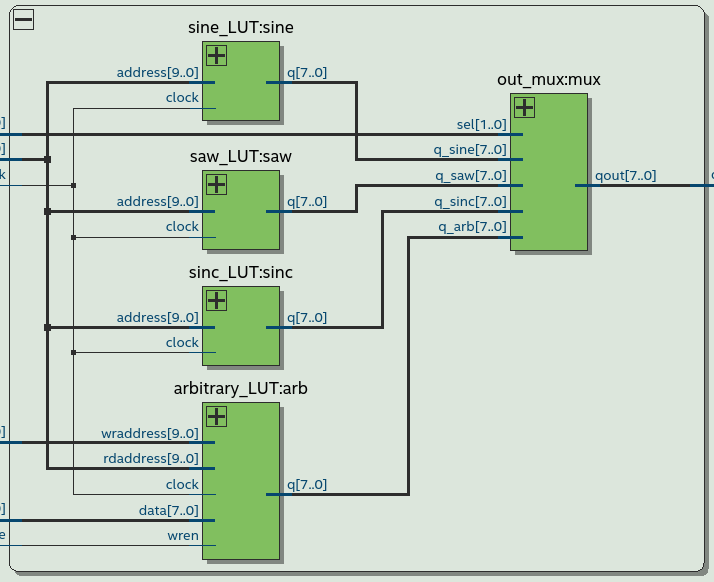
\includegraphics[width=0.75\textwidth]{./figuras/rtl_LUT}
	\legend{Fonte~---~Autoria própria.}
\end{figure}

A Figura~\ref{fig:tb_lut} mostra, para cada memória, o valor lido em cada um dos 1024 endereços, percorridos em ordem embaralhada, sobre o conteúdo esperado dos arquivos \ac{mif}. As seis varreduras terminaram sem nenhuma diferença. A varredura (e) foi feita com a escrita de um novo padrão em toda a \ac{ram} ao mesmo tempo, e confirma que a escrita não perturba a leitura das outras tabelas; a varredura (f) confirma que a \ac{ram} devolve o padrão escrito, três períodos de uma senoide. A Figura~\ref{fig:tb_lut_lat} mostra a latência de dois clocks entre o endereço e a amostra.

\begin{figure}
	\caption{Leitura das quatro memórias, endereço a endereço, comparada com o conteúdo esperado.}
	\label{fig:tb_lut}
	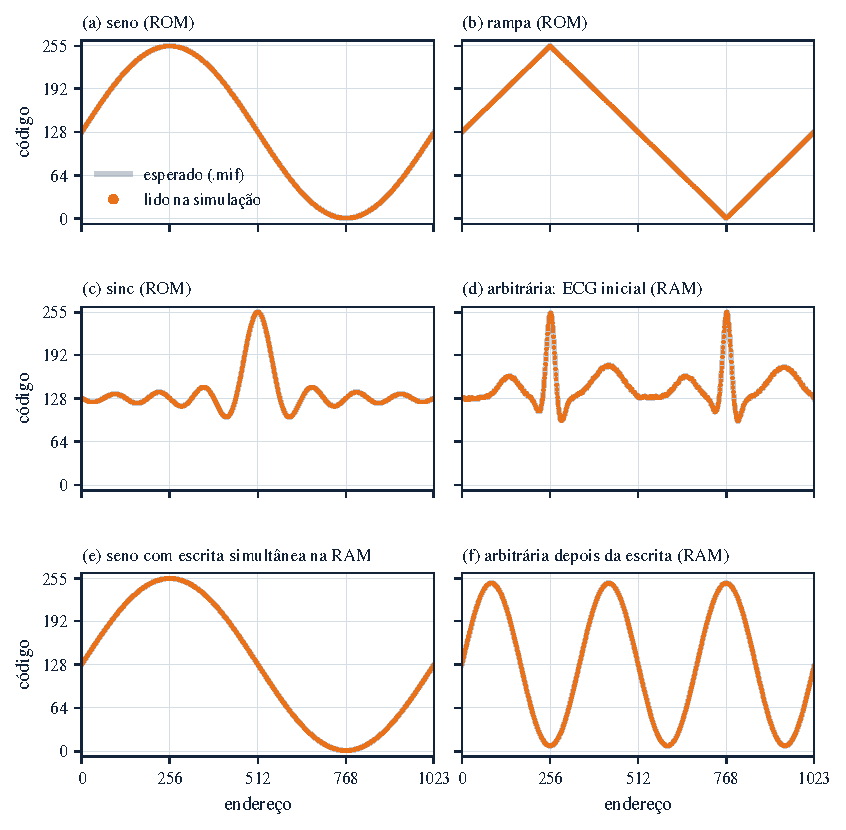
\includegraphics[width=\textwidth]{./figuras/tb_LUT_tabelas}
	\legend{Fonte~---~Autoria própria.}
\end{figure}

\begin{figure}
	\caption{Latência de dois clocks entre o endereço e a amostra nas memórias.}
	\label{fig:tb_lut_lat}
	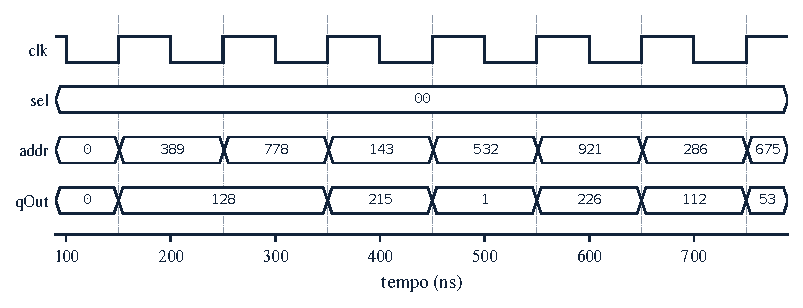
\includegraphics[width=\textwidth]{./figuras/tb_LUT_latencia}
	\legend{Fonte~---~Autoria própria.}
\end{figure}

\subsection{Núcleo DDS}

A Figura~\ref{fig:rtl_core} mostra o núcleo no RTL, com os três blocos ligados em sequência: acumulador de fase, tabelas e registrador de saída.

\begin{figure}
	\caption{Visão RTL do núcleo \acs{dds} (\cod{dds\_core}).}
	\label{fig:rtl_core}
	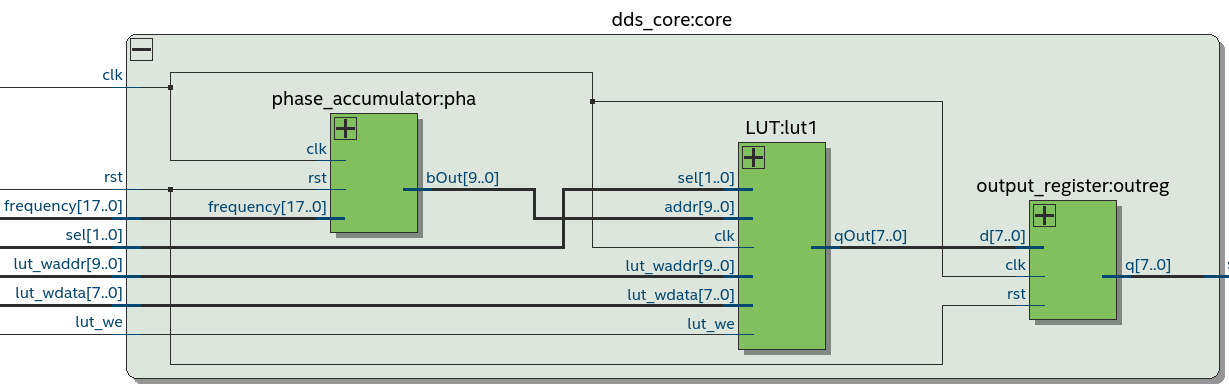
\includegraphics[width=\textwidth]{./figuras/rtl_dds_core}
	\legend{Fonte~---~Autoria própria.}
\end{figure}

O \eng{testbench} do núcleo \cod{dds\_core} comparou 14\,034 amostras de saída com o modelo de referência, sem nenhuma diferença. A Figura~\ref{fig:tb_core} mostra trechos da saída em cada situação testada. Na Figura~\ref{fig:tb_core}(b), a frequência muda de 100~kHz para 262\,143~Hz no instante marcado pela linha tracejada, e o sinal continua sem descontinuidade. Na Figura~\ref{fig:tb_core}(f), a forma de onda é um dente de serra escrito na \ac{ram} enquanto o seno estava na saída.

\begin{figure}
	\caption{Saída do núcleo \acs{dds} para as quatro formas de onda, na troca de frequência e após a escrita da tabela arbitrária.}
	\label{fig:tb_core}
	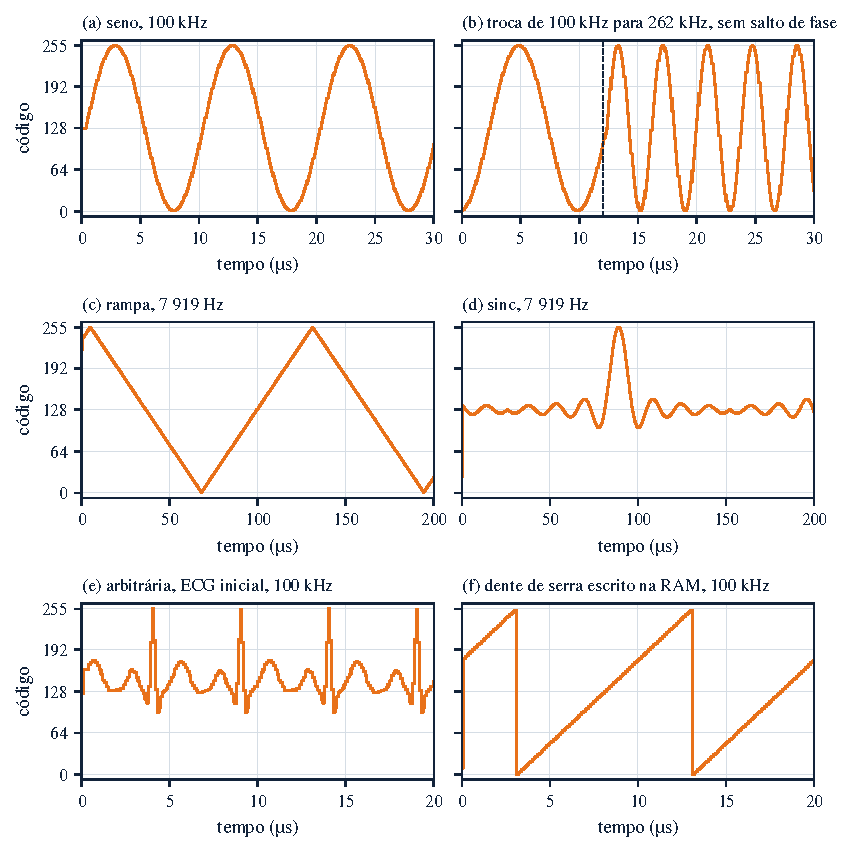
\includegraphics[width=\textwidth]{./figuras/tb_dds_core_formas}
	\legend{Fonte~---~Autoria própria.}
\end{figure}

A Figura~\ref{fig:tb_core_lat} mostra a saída do \eng{reset} em 100~kHz. Durante o \eng{reset}, a amostra permanece em 128, o zero do sinal. Depois dele, o endereço avança 10 posições por clock (\(100~\text{kHz} \cdot 1024/10~\text{MHz} \approx 10{,}24\)), e cada endereço aparece na saída três clocks depois, como previsto.

\begin{figure}
	\caption{Saída do \eng{reset} no núcleo \acs{dds}: latência de três clocks entre o endereço e a amostra.}
	\label{fig:tb_core_lat}
	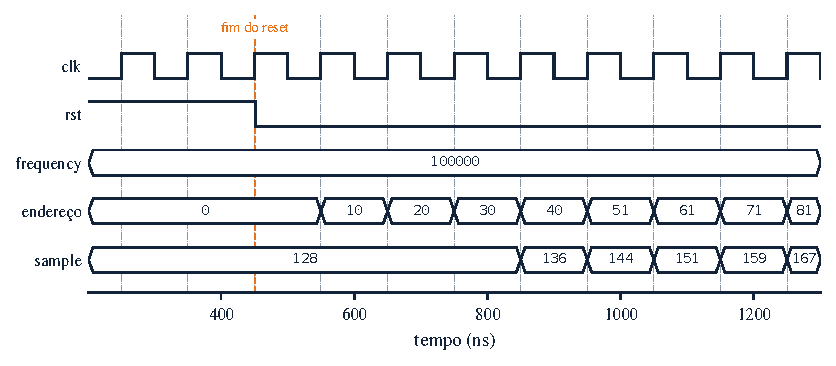
\includegraphics[width=\textwidth]{./figuras/tb_dds_core_latencia}
	\legend{Fonte~---~Autoria própria.}
\end{figure}

\section{Verificação do controle pelo computador}

\pendente{Inserir a visão RTL do \cod{vjtag\_dr} (caminho \cod{pc}, \cod{ctrl}, \cod{dr} no RTL Viewer).}

A Figura~\ref{fig:tb_vjtag} mostra dois comandos de frequência no bloco \cod{vjtag\_dr}. Em cada um, o Capture-DR é seguido de 18 ciclos de Shift-DR, em que os bits entram por \cod{tdi}, com o \ac{lsb} primeiro, e o registrador \cod{dr} se forma. No Update-DR, o valor é copiado para \cod{cmd\_data} e \cod{cmd\_toggle} muda de nível. Durante o segundo deslocamento, \cod{tdo} devolve o valor do primeiro comando (\cod{2A5A5}), carregado no Capture-DR, o que permite ler a configuração.

\begin{figure}
	\caption{Dois comandos de frequência no registrador de dados do Virtual \acs{jtag}.}
	\label{fig:tb_vjtag}
	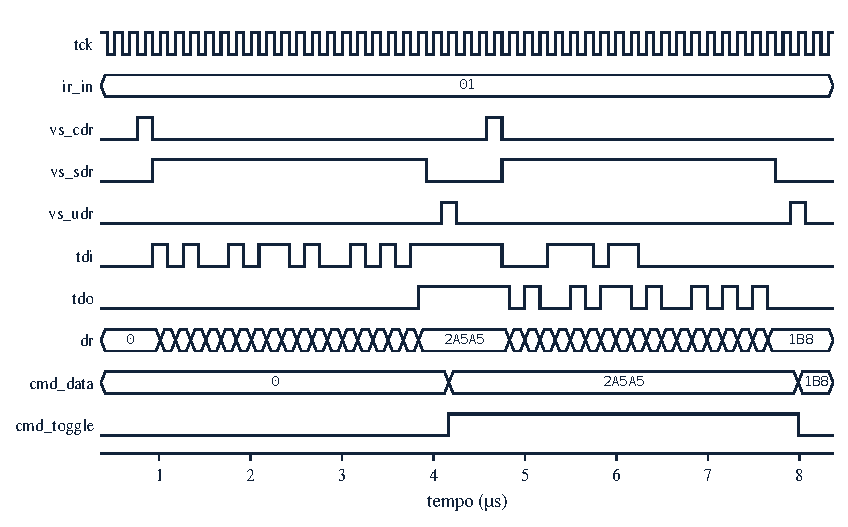
\includegraphics[width=\textwidth]{./figuras/tb_vjtag_dr}
	\legend{Fonte~---~Autoria própria.}
\end{figure}

A Figura~\ref{fig:rtl_cmd_sync} mostra o \cod{cmd\_sync} no RTL: a cadeia de três \eng{flip-flops} do sincronizador (\cod{sync}), o registrador \cod{last}, que guarda o último nível visto, a comparação entre os dois e os registradores de saída \cod{valid} e \cod{data}.

\begin{figure}
	\caption{Visão RTL da passagem de comandos entre domínios de clock (\cod{cmd\_sync}).}
	\label{fig:rtl_cmd_sync}
	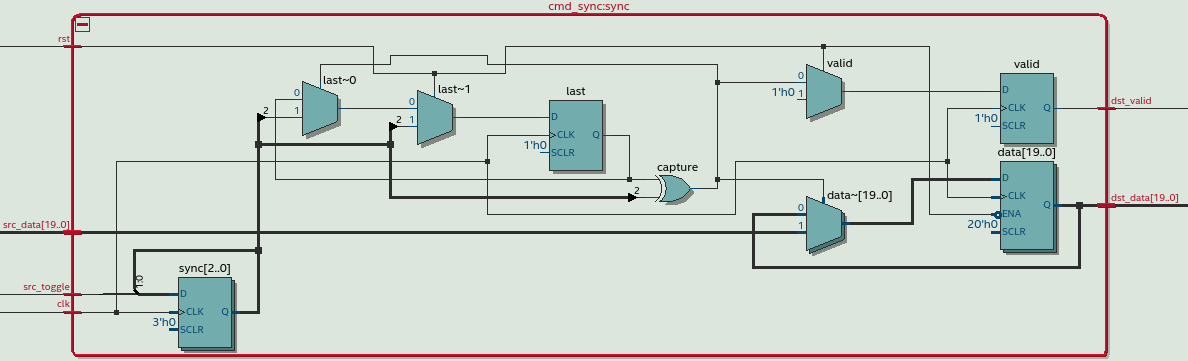
\includegraphics[width=\textwidth]{./figuras/rtl_cmd_sync}
	\legend{Fonte~---~Autoria própria.}
\end{figure}

A Figura~\ref{fig:tb_cmd_sync} mostra a passagem de um comando para o domínio de 10~MHz. A mudança de \cod{src\_toggle} percorre os três \eng{flip-flops} do sincronizador; quando chega ao último, o dado é copiado para \cod{dst\_data} e \cod{dst\_valid} pulsa por um clock. No \eng{testbench}, 300 comandos com dados e intervalos aleatórios, gerados por um clock de 6~MHz sem relação de fase com o de destino, foram entregues uma única vez, em ordem e com o dado correto, e um \eng{reset} no destino não repetiu nenhum comando.

\begin{figure}
	\caption{Passagem de um comando do domínio do \cod{tck} para o de 10~MHz.}
	\label{fig:tb_cmd_sync}
	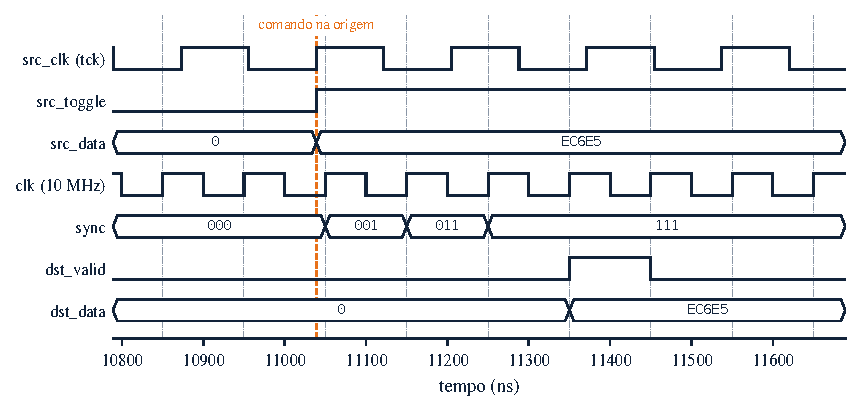
\includegraphics[width=\textwidth]{./figuras/tb_cmd_sync}
	\legend{Fonte~---~Autoria própria.}
\end{figure}

A Figura~\ref{fig:rtl_jtag} mostra o \cod{jtag\_control} no RTL, com os três blocos: \cod{vjtag\_dr}, \cod{cmd\_sync} e \cod{control\_registers}. O comando de 20~bits sai do \cod{vjtag\_dr}, atravessa o \cod{cmd\_sync} e é separado em instrução e dado na entrada dos registradores.

\begin{figure}
	\caption{Visão RTL do controle pelo computador (\cod{jtag\_control}).}
	\label{fig:rtl_jtag}
	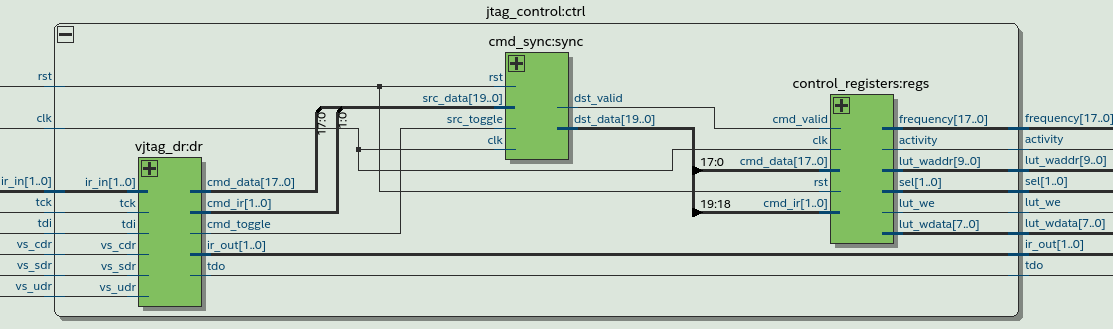
\includegraphics[width=\textwidth]{./figuras/rtl_jtag_control}
	\legend{Fonte~---~Autoria própria.}
\end{figure}

A Figura~\ref{fig:tb_jtag} mostra o caminho completo de um comando de 440~Hz no bloco \cod{jtag\_control}: do deslocamento no domínio do \cod{tck} até o registrador de frequência no domínio de 10~MHz. O registrador é atualizado 566~ns após o Update-DR, um tempo muito menor que o de um novo deslocamento. No mesmo \eng{testbench}, 64 escritas consecutivas na tabela geraram 64 pulsos de escrita, na ordem e com os endereços e dados corretos.

\begin{figure}
	\caption{Comando de frequência do registrador de dados do \acs{jtag} até o registrador de frequência.}
	\label{fig:tb_jtag}
	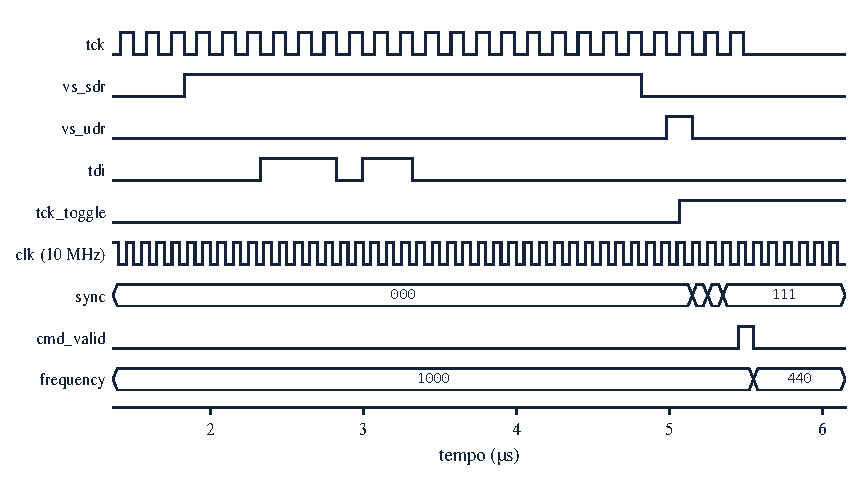
\includegraphics[width=\textwidth]{./figuras/tb_jtag_control}
	\legend{Fonte~---~Autoria própria.}
\end{figure}

\section{Verificação do sistema}

A Figura~\ref{fig:rtl_dds} mostra a entidade do topo no RTL. Ela contém apenas as ligações entre o \ac{pll}, o \cod{reset\_sync}, o \cod{jtag\_interface} e o \cod{dds\_core}, além da porta OU que combina o botão de \eng{reset} com a indicação de travamento do \ac{pll}.

\begin{figure}
	\caption{Visão RTL da entidade do topo (\cod{DDS}).}
	\label{fig:rtl_dds}
	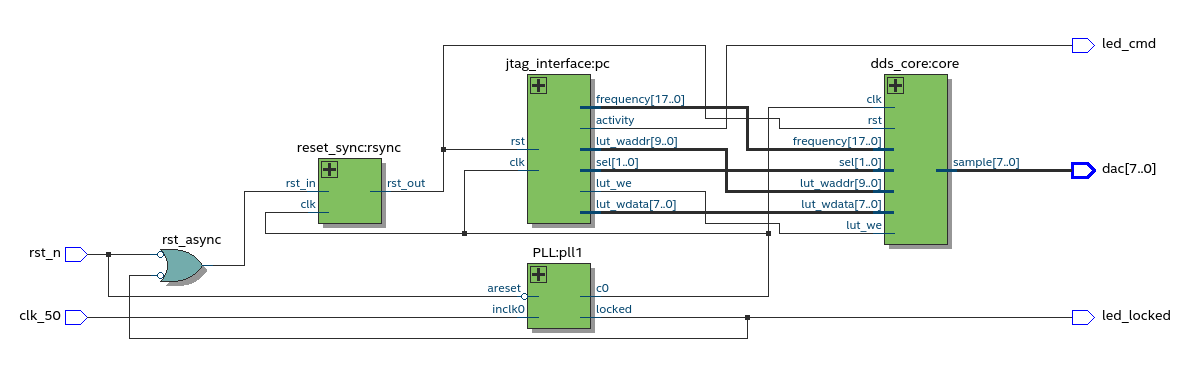
\includegraphics[width=\textwidth]{./figuras/rtl_DDS}
	\legend{Fonte~---~Autoria própria.}
\end{figure}

O \eng{testbench} \cod{tb\_system} reúne o controle e o núcleo e faz o papel do computador, enviando a mesma sequência de comandos que a interface gráfica enviaria. A Figura~\ref{fig:tb_sys} mostra a saída durante toda a simulação. Após o \eng{reset}, sem nenhum comando, o gerador produz o seno de 1~kHz. Em seguida, o computador pede 100~kHz e seno, depois sinc, envia uma tabela inteira, com 1024 escritas, e escolhe a forma arbitrária em 50~kHz. A Figura~\ref{fig:tb_sys_det}(a) mostra o momento em que o comando de frequência chega, e a Figura~\ref{fig:tb_sys_det}(b), a tabela enviada sendo reproduzida. Em cada trecho, cada amostra foi comparada com a tabela correspondente, e a frequência medida pelas voltas do endereço coincidiu com a pedida, dentro da tolerância de 0,1\% usada no \eng{testbench}.

\begin{figure}
	\caption{Saída do sistema durante a sequência de comandos do computador.}
	\label{fig:tb_sys}
	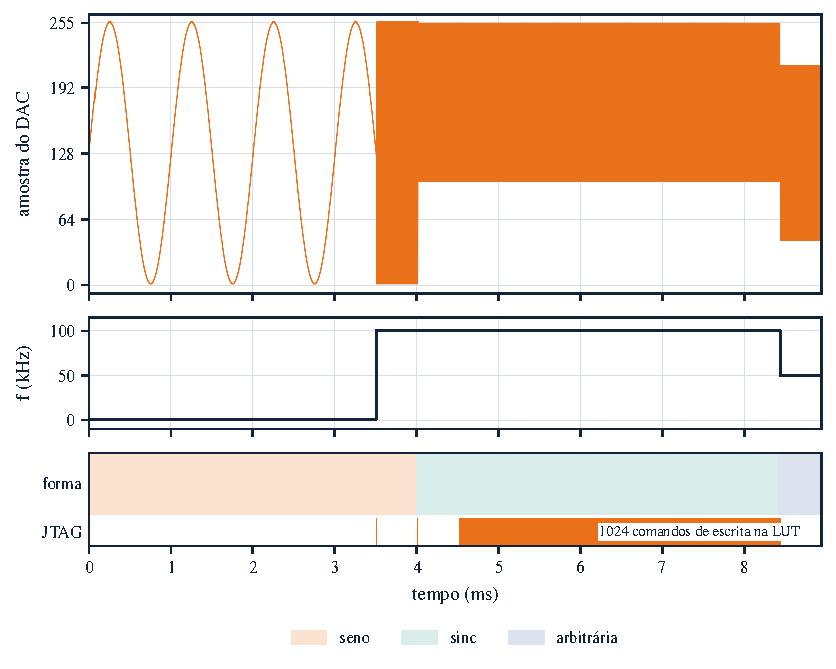
\includegraphics[width=\textwidth]{./figuras/tb_system_visao_geral}
	\legend{Fonte~---~Autoria própria.}
\end{figure}

\begin{figure}
	\caption{Detalhes da simulação do sistema: (a) chegada do comando de frequência; (b) tabela enviada pelo \acs{jtag} reproduzida na saída.}
	\label{fig:tb_sys_det}
	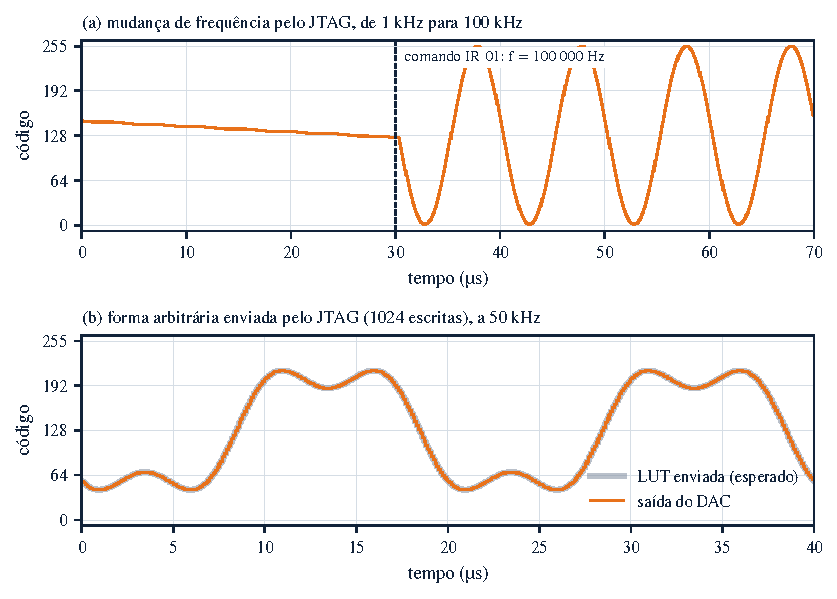
\includegraphics[width=\textwidth]{./figuras/tb_system_detalhes}
	\legend{Fonte~---~Autoria própria.}
\end{figure}

Por fim, o \eng{testbench} \cod{tb\_DDS} simula a entidade do topo, com o \ac{pll} e as memórias pelos modelos da Intel. A Figura~\ref{fig:tb_pll} mostra o travamento do \ac{pll}: o clock de 10~MHz surge, o \eng{LED} de travamento acende e o \eng{reset} interno é liberado três clocks depois. A Figura~\ref{fig:tb_dds} mostra os pinos do \ac{dac}: o seno de 1~kHz após a liberação do botão e o retorno ao código 128 quando o botão é pressionado novamente. A frequência medida nos pinos ficou dentro de 1~Hz de 1~kHz, a tolerância usada no \eng{testbench}.

\begin{figure}
	\caption{Travamento do \acs{pll} e liberação do \eng{reset} interno na entidade do topo.}
	\label{fig:tb_pll}
	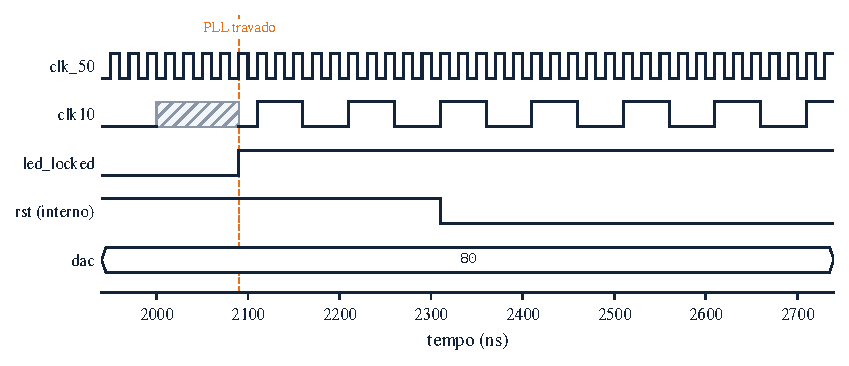
\includegraphics[width=\textwidth]{./figuras/tb_DDS_pll}
	\legend{Fonte~---~Autoria própria.}
\end{figure}

\begin{figure}
	\caption{Código nos pinos do \acs{dac} na simulação da entidade do topo.}
	\label{fig:tb_dds}
	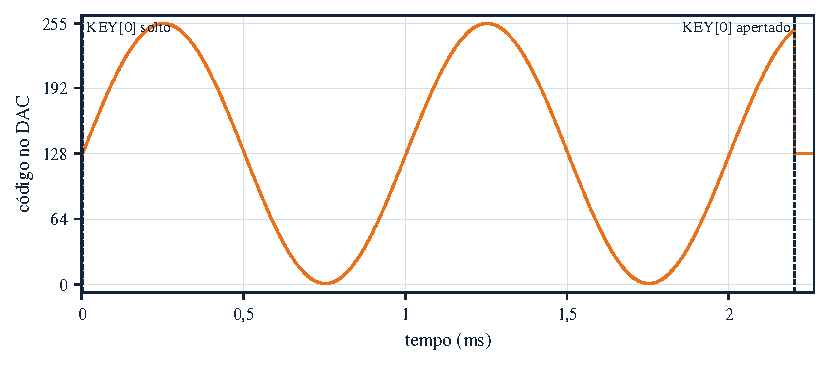
\includegraphics[width=\textwidth]{./figuras/tb_DDS_saida}
	\legend{Fonte~---~Autoria própria.}
\end{figure}

\section{Simulação da placa analógica}

A simulação no LTspice cobre 5~ms, ou cinco períodos do seno de 1~kHz produzido pelo \ac{vhdl}. A Figura~\ref{fig:spice_tempo}(a) mostra a tensão na saída do conversor corrente-tensão e na saída final, depois do ganho, do filtro e do \eng{buffer}; a inversão de fase entre as duas vem do amplificador inversor. A Tabela~\ref{tab:spice} compara os valores obtidos com os calculados no Capítulo~\ref{cap:metodologia}, e todos coincidem. A tensão correspondente ao código 128 não é exatamente zero: como \(I_{FS} = I_{REF} \cdot 255/256\), pela Equação~(\ref{eq:dac0800}), o código 128 dá \(I_{OUT} - \overline{I_{OUT}} = I_{REF}/256\), ou 7,81~mV na saída do conversor.

\begin{table}
	\caption{Valores obtidos na simulação do circuito analógico.}
	\label{tab:spice}
	\begin{tabular}{l c c}\toprule
		Grandeza & Simulado & Calculado\\\midrule
		Corrente de escala completa do \acs{dac} & 1,99~mA & 1,992~mA\\
		Excursão do conversor corrente-tensão & \(-1{,}976\) a \(+1{,}991\)~V & \(-1{,}977\) a \(+1{,}992\)~V\\
		Tensão do código 128 no conversor & 7,81~mV & 7,81~mV\\
		Ganho do estágio inversor & \(-1{,}19999\) & \(-1{,}2\)\\
		Excursão da saída & 4,760~V de pico a pico & 4,763~V de pico a pico\\
		Frequência & 1,000~kHz & 999,998~Hz\\
		Atraso do filtro em 1~kHz & 321~ns & 317~ns\\\bottomrule
	\end{tabular}
	\legend{Fonte~---~Autoria própria.}
\end{table}

A Figura~\ref{fig:spice_tempo}(b) mostra o efeito do filtro de reconstrução em uma subida do seno. Antes do filtro, a saída é uma escada: em 1~kHz, cada código dura cerca de 1~\(\mu\)s e cada degrau tem 18,75~mV, um \ac{lsb} multiplicado pelo ganho. Depois do filtro, as transições ficam suavizadas e atrasadas em 321~ns. Esse atraso concorda com o atraso de grupo de um filtro de segunda ordem em baixa frequência, \(1/(Q\,\omega_0) \approx 317\)~ns, e não depende da forma de onda.

\begin{figure}
	\caption{Simulação da placa analógica para o seno de 1~kHz: (a) saídas do conversor corrente-tensão e do circuito; (b) detalhe de uma subida, antes e depois do filtro.}
	\label{fig:spice_tempo}
	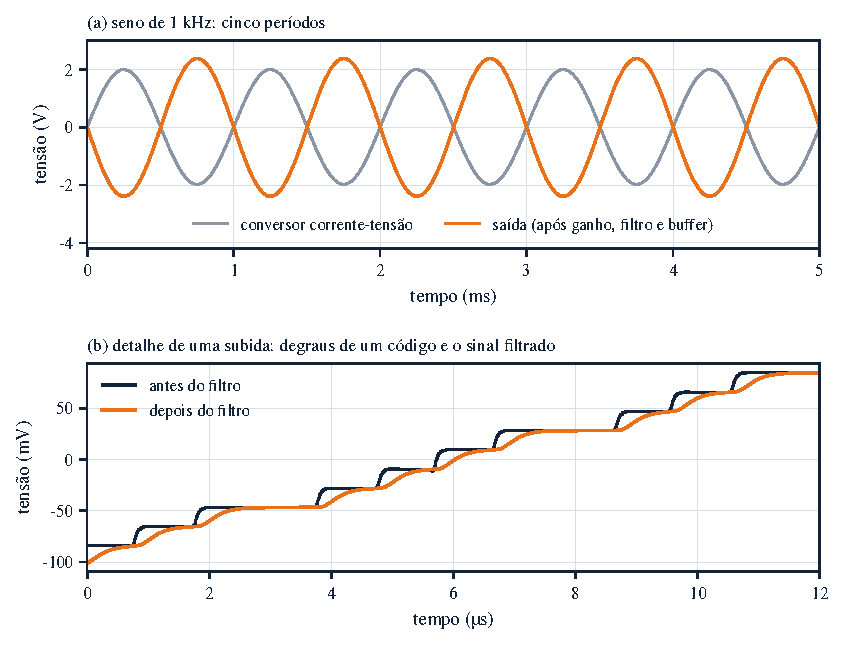
\includegraphics[width=\textwidth]{./figuras/spice_tempo}
	\legend{Fonte~---~Autoria própria.}
\end{figure}

A Figura~\ref{fig:spice_fft} mostra o espectro dos dois pontos, calculado pelo LTspice com resolução de 200~Hz e normalizado pela componente de 1~kHz. Aparecem três grupos de componentes, todos previstos no Capítulo~\ref{cap:teoria}:
\begin{description}
	\item[Harmônicas] --- principalmente ímpares, com a maior, a 9.ª, em \(-73{,}4\)~dBc, e distorção harmônica total, da 2.ª à 10.ª, de \(-70{,}9\)~dBc. Elas vêm da quantização em 8~bits: como o período tem exatamente 1024 amostras, o erro de quantização se repete a cada período e se concentra em harmônicas, em vez de se espalhar como ruído. O filtro não as altera, pois estão dentro da banda passante;
	\item[Imagens da tabela] --- em \(1024 f_{out} \pm f_{out}\) (1,023 e 1,025~MHz). Em 1~kHz, a saída é uma escada de 1024 degraus por período, atualizada a 1,024~MHz, e a Equação~(\ref{eq:zoh}) passa a valer com essa taxa no lugar de \(f_{clk}\). Essa é a maior componente indesejada: \(-60{,}5\)~dBc antes do filtro, em acordo com o limite de \(6{,}02\,P\) da Equação~(\ref{eq:sfdr}), e \(-67{,}0\)~dBc depois, pois o filtro atenua cerca de 6~dB em \(f_0\), como esperado para \(Q = 0{,}5\);
	\item[Imagens do clock] --- em \(f_{clk} \pm f_{out}\), em \(-96\)~dBc antes do filtro e \(-119\)~dBc depois, já próximas do piso numérico da simulação. Nesse ponto, a envoltória sinc da Equação~(\ref{eq:zoh}) vale cerca de \(f_{out}/f_{clk}\), ou \(-80\)~dB, e as transições do \acs{dac} e a banda limitada dos amplificadores atenuam um pouco mais.
\end{description}

\begin{figure}
	\caption{Espectro da simulação da placa analógica para o seno de 1~kHz, antes e depois do filtro de reconstrução.}
	\label{fig:spice_fft}
	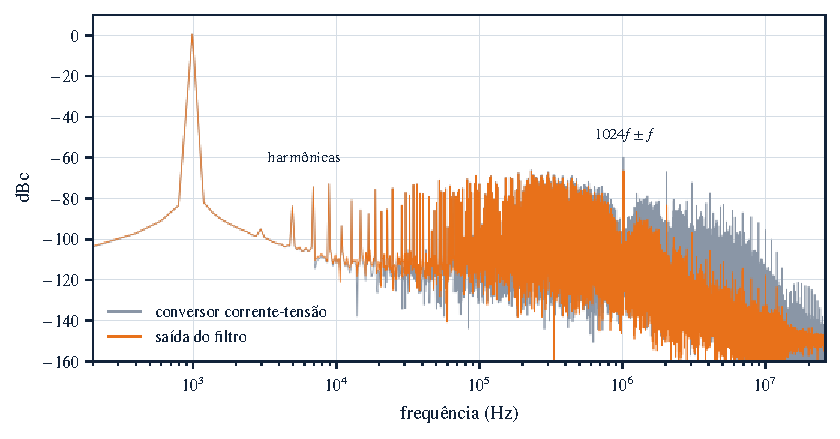
\includegraphics[width=\textwidth]{./figuras/spice_fft}
	\legend{Fonte~---~Autoria própria.}
\end{figure}

\section{Ensaios em bancada}

A Figura~\ref{fig:bancada} mostra a montagem de bancada: a DE2-115, a placa analógica ligada ao conector de expansão, as fontes de \(\pm15\)~V e +10~V e o osciloscópio. Uma medição preliminar da placa analógica, feita em 3 de setembro de 2026 com uma versão anterior do código do \ac{fpga}, é mostrada na Figura~\ref{fig:medicao}: um seno de 100,0~Hz com 5,08~V de pico a pico. \pendente{Confirmar a versão do código usada nessa medição.}

\begin{figure}
	\caption{Montagem de bancada.}
	\label{fig:bancada}
	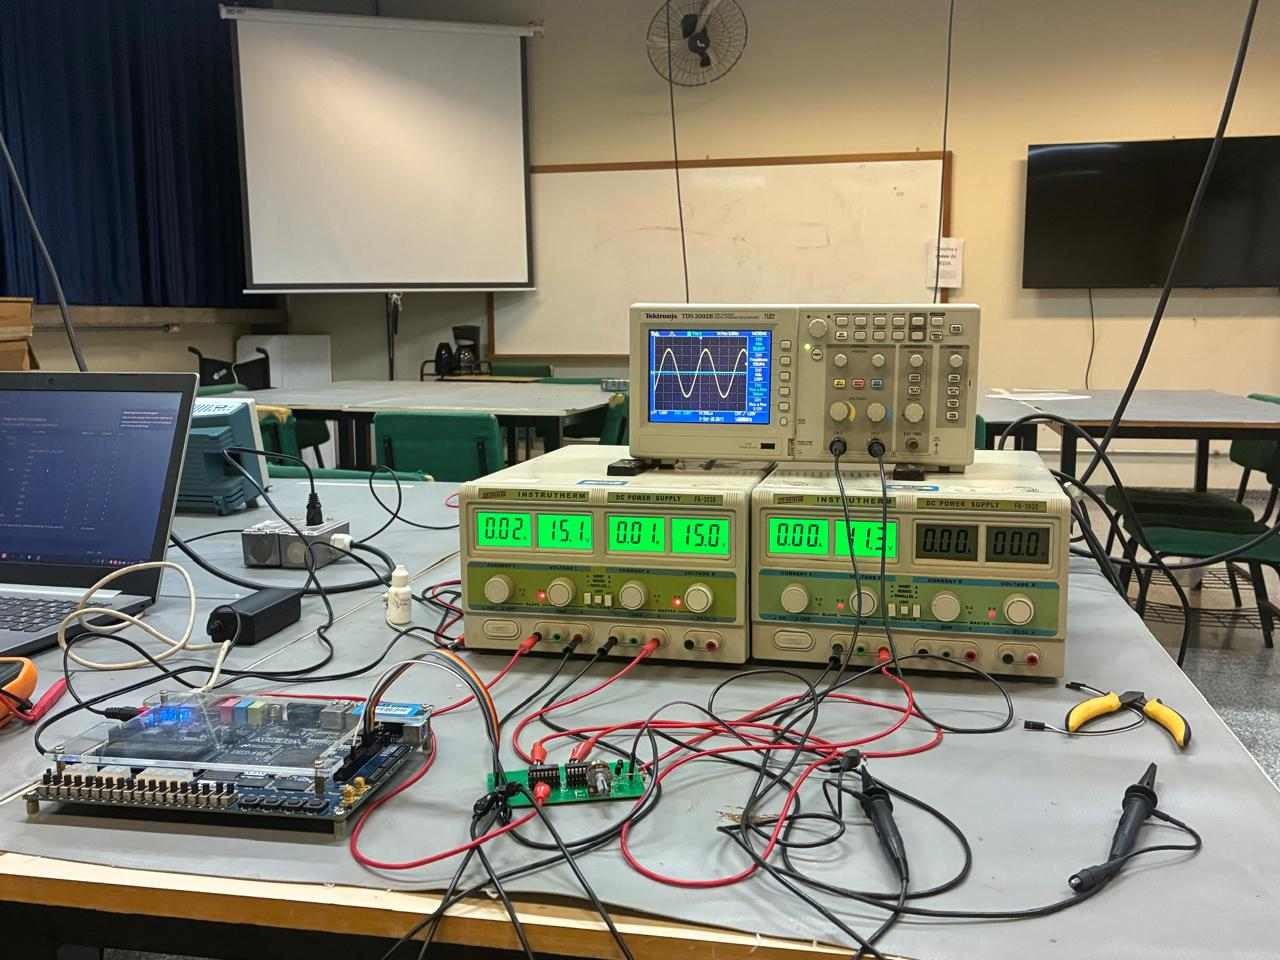
\includegraphics[width=0.8\textwidth]{./figuras/bancada}
	\legend{Fonte~---~Autoria própria.}
\end{figure}

\begin{figure}
	\caption{Medição preliminar na saída da placa analógica: seno de 100,0~Hz com 5,08~V de pico a pico.}
	\label{fig:medicao}
	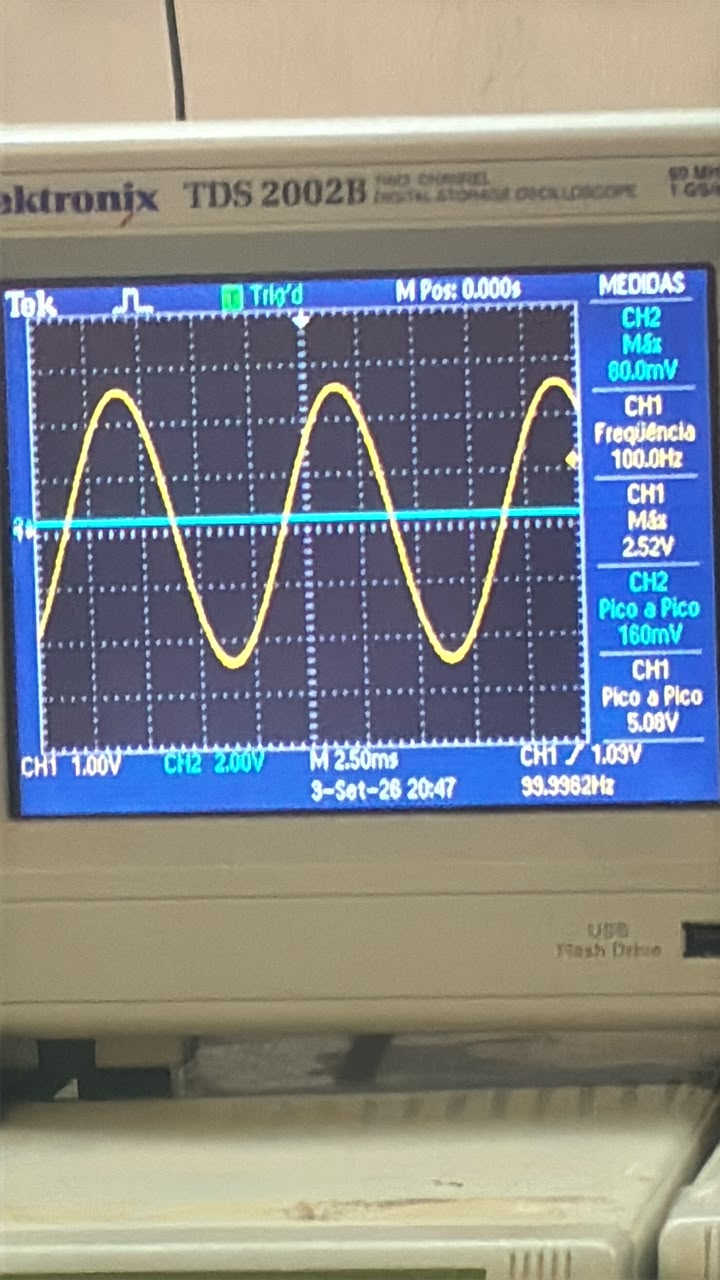
\includegraphics[width=0.5\textwidth]{./figuras/medicao}
	\legend{Fonte~---~Autoria própria.}
\end{figure}

\pendente{Ensaios com o código final: controle pela interface gráfica; frequência medida em vários pontos da faixa; as quatro formas de onda e o envio de uma tabela arbitrária; amplitude e ajuste de ganho; e espectro da saída, para comparar o maior espúrio com a Figura~\ref{fig:espectros}.}
